\documentclass[a4paper,10pt,francais]{article}
    \usepackage[T1]{fontenc}
    \usepackage[ansinew]{inputenc}
    \usepackage{graphicx}
    \usepackage{babel}
    \usepackage{amssymb}
	\usepackage{textcomp}
	\usepackage{bm}
	\usepackage{authblk}
	\usepackage{amsmath}
%%% Mise en page
\setlength{\hoffset}{-0.75in} \setlength{\voffset}{-0.50in}
\setlength{\topmargin}{0cm} \setlength{\headheight}{0cm}
\setlength{\headsep}{1cm} \setlength{\textwidth}{17cm}
\setlength{\textheight}{26.5cm} \setlength{\footskip}{0cm}
\pagestyle{empty} \everymath{\displaystyle}

%%% Compteurs
\newcounter{exo}
\newcommand{\nvexo}{
\stepcounter{exo} \vspace{0.2cm} \noindent
                  \textbf{Exercice n${}^o$\theexo}\hrulefill \\
                       }

\newcommand{\R}{\mathbb{R}}
\newcommand{\C}{\mathbb{C}}
\newcommand{\N}{\mathbb{N}}
\newcommand{\Z}{\mathbb{Z}}
\newcommand{\Q}{\mathbb{Q}}
\newcommand{\et}{\textrm{ et }}
\newcommand{\ou}{\textrm{ ou }}
\newcommand{\non}{\textrm{non }}
\newcommand{\ssi}{si et seulement si }
\newcommand{\ch}{\mathrm{ch }\, }
\newcommand{\sh}{\mathrm{sh }\, }
\newcommand{\tnh}{\mathrm{th }\, }
\newcommand{\pgcd}{\mathrm{pgcd} }
\newcommand{\ppcm}{\mathrm{ppcm} }
\newcommand{\com}{\mathrm{com} }
\newcommand{\rg}{\mathrm{rg} }
\newcommand{\val}{\mathrm{val} }
\newcommand{\Argch}{\mathrm{Argch }\, }
\newcommand{\Argsh}{\mathrm{Argsh }\, }
\newcommand{\Argth}{\mathrm{Argth }\, }
\newcommand{\Arcsin}{\mathrm{Arcsin }\, }
\newcommand{\Arccos}{\mathrm{Arccos }\, }
\newcommand{\Arctan}{\mathrm{Arctan }\, }
\newcommand{\rd}[1]{\overset{\; \circ}{#1}}
\newcommand{\br}[1]{\overline{#1}}
\newcommand{\un}{$(u_n)_{n \in \N}$}
\newcommand{\card}{\mathrm{Card}}
\newcommand{\re}{\textrm{Re }}
\newcommand{\im}{\textrm{Im }}
\newcommand{\pr}{{\bf Preuve.} }
\newcommand{\vect}[1]{\overrightarrow{#1}}
\newcommand{\boite}[1]{\framebox[1.1\width]{#1}}
\newcommand{\voca}{ \section{Vocabulaire de la le�on}}
\newcommand{\dr}{\begin{quote}}
\newcommand{\fr}{\end{quote}}


%%% Abreviations
\let\leq=\leqslant \let\geq=\geqslant
\let\sm=\setminus
\let\wt=\widetilde
\let\wh=\widehat
\let \l=<
\let \g=>
\newtheorem{thm}{Th�or�me}
\newcommand{\cqfd}{\hfill $\Box$}
\newcommand{\sern}{\sum_{n=1}^{\infty}}
\pagestyle{myheadings}
\markright{{\footnotesize \'Ecole Centrale de Lyon - LMFA}}

%%%%%%%%%%%%%%%%%%%%%%%%%%%%%%%%%%%%%%%%%%%%%%%%%%%%%%%%%%%%%%%%
\title{How Planes Fly}
\author[1]{David Louapre}
\affil[1]{https://sciencetonnante.wordpress.com/2016/09/25/comment-un-avion-vole-t-il/}
\author[2]{Dr Goulu}
\affil[2]{https://www.drgoulu.com/2012/03/11/portance-pourquoi-ca-vole/\#.WcXzI8gjGM8}
\author[3]{Couleur Science}
\affil[3]{https://couleur-science.eu/?d=2016/09/15/22/46/21-comment-vole-un-avion-et-non-ce-nest-pas-juste-bernoulli}
\renewcommand\Affilfont{\itshape\small}

\begin{document}
\parindent=0cm
\parskip=3mm

\maketitle


\section{Quick Answer}

Coanda Effect makes planes fly.


\section{notes and memory}

Bernoulli theorem is often taken as/talked about concerning lifts. Its explication is like : air on the top has a longer distance to travel whereas on the bottom air moves more slowly. Where the fluid flows slowlier, where the pressure got higher. Therefore a pressure difference is created thus lift.\\


\begin{figure}[h!]
\centering
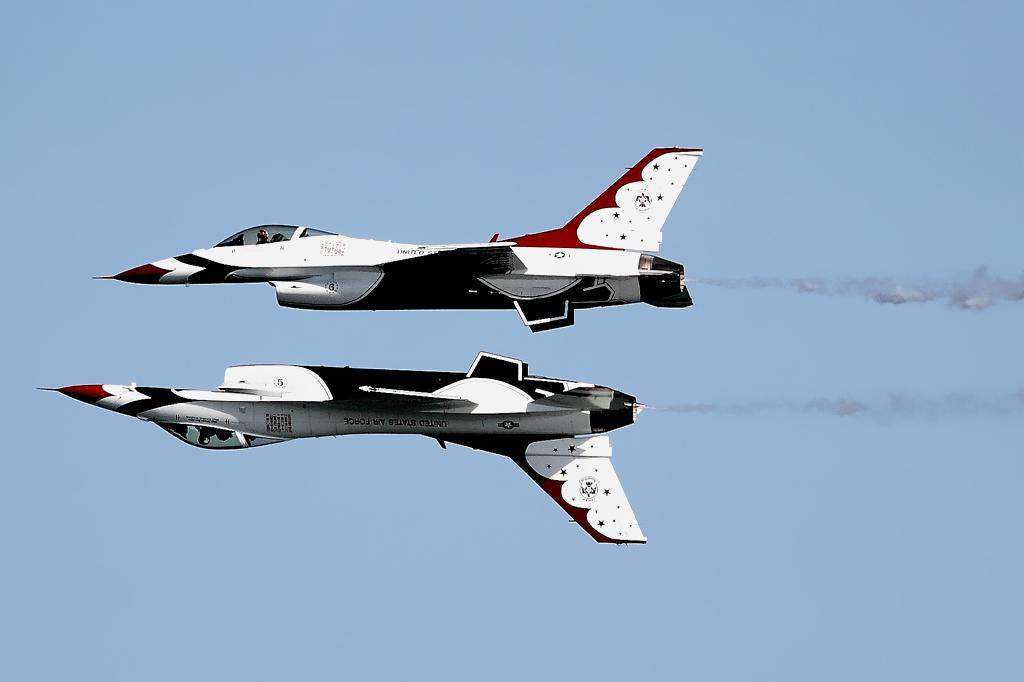
\includegraphics[width=0.49\textwidth]{Wrong-Bernouilli}
\caption{\label{fig:1} The pressure difference just don't count that much in lift}
\end{figure}


Have a look at Fig\ref{fig:1}, trival isn't it?! In reality, lift created by this pressure difference is minor. Whereas a Newton's law seem to apply when taking the flow over airfoil as a whole : the fluid is derived by airfoil {\it somehow (actually by coanda effect)} getting a momentum downwards thus giving airplane a momentum upwards.\\

When angle of attack is not steep (too big), the fluid seems to be tamed and derived downwards passing by airfoil.\\

Slats and flags are used when the civil plane is taking off or landing in order to enhance the coanda effect thus enhance lifts. Fighters do that to cruise at lower speed favoring a quick turn.


\section{Annexe : some Eqs on momentum changing rate}

The momentum of air in a volume that includes volume of the airfoil at instant $t$ (assuming $\rho$ is constant and flow is stationnary for now, so the change will only come from flux/convection):
$$\vec{p} = \iiint_V \rho\vec{v}(\vec{x}) d\tau$$
At $t+\Delta t$
$$\vec{p'} = \iiint_V \rho\vec{v}(\vec{x}) d\tau$$
Momentum change rate:
$$\vec{F}=\frac{d\vec{p}}{dt}= \lim_{\Delta t \to 0} \iiint_V \rho (\frac{\vec{v}(\vec{x}+\vec{v}\Delta t) - \vec{v}(\vec{x})}{\Delta t}) d\tau$$
Which is a direction derivative of $\vec{v}$ in direction $\vec{v}$ (See Pauly's G�ometrie 2):
$$\frac{d\vec{p}}{dt}= \iiint_V \rho(\vec{v} \cdot \vec{\nabla} \vec{v}) d\tau$$
Taking the instationnarity into account, we obtain then
$$\frac{d\vec{p}}{dt}= \iiint_V \rho(\frac{\partial\vec{v}}{\partial t} + \vec{v} \cdot \vec{\nabla} \vec{v}) d\tau = \iiint_V \rho \frac{D\vec{v}}{Dt} d\tau$$
Where a total derivative $\frac{d}{dt}$ or material derivative $\frac{D}{Dt}$ is applied. \\

Take one step back and think of Newton's second law in high school which only involves one derivative $\frac{d}{dt}$ which is Lagrangian. Here in fluid mechanics we have total derivative $\frac{d}{dt}$ or material derivative $\frac{D}{Dt}$ for a control volume which is itself static in the case above (if not, Reynolds Theorem applies where the time variation of the control volume is taken into account). What differentiate from high school material point mechanics and fluid mechanics is the presence of flux in and flux out. Mathmatically speaking, we interprate material point with Lagrangian representation and flow with Eularian representation : the $\frac{d}{dt}$ in high school is indeed a material derivative in term of material though there's no flux; $\frac{d}{dt}$ or $\frac{D}{Dt}$ in fluid mechanics are always applied to volumes instead of material points (which is consistent, because $\Delta \tau$ is small but remains a volume) though very often called "fluid particles". And $\frac{Du}{Dt}$ is a Lagrangian quantity (Lagrangian accelaration) dependant on a Eularian variable. $u(\vec{x},t)$. {\bf So in one word, N-S equation is a Lagrangian Newton's second law translated in Eularian variables which as a consequence involves convective/nonlinear term}.

\end{document}
